\SetPicSubDir{ch-Exp}

\chapter{Experimenting with Other Random Models}
\label{ch:exp}
\vspace{2em}

A method similar to the 3-phase method in DHAM has been adopted and used to show existential/constructive results in some other models of random digraphs. Now that we are familiar with the DHAM algorithms, we shall attempt to inpnut graphs from some of these models, and see how DHAM performs on them. We shall try to look for patterns in terms of accuracy, runtime, or number of attempts in the following models.

\section{$k$-in, $k$-out Graphs}
\subsection{Graph Generation}
The way $D_{k-in, k-out}$ is defined, it is pretty straightforward to generate instances of this graph. At every vertex $u\in V_n$, we simply have to generate 2 lists of $k$ vertices each (as in-neighbours and out-neighbours), sampling uniformly at random from the set of all vertices. Now we add an edge from $u$ to each out-neighbour and an edge from each in-neighbour to $u$.
\subsection{Observations}
Cooper and Frieze \cite{cooper:kinout} have shown that $D_{2-in, 2-out}$ is Hamiltonian with High Probability, using a 3-phase analysis. 

\begin{description}
\item[Phase 1] Show that $D_{2-in, 2-out}$ contains a permutation digraph, $\Pi$ of size at most $2\log n$.
\item[Phase 2] Increase the minimum cycle length in $\Pi$ to $n_0 = \Big\lceil \frac{1000n}{\log n} \Big\rceil$.
\item[Phase 3] Convert the Phase 2 permutation digraph to a Hamilton Cycle.
\end{description}
It is interesting to note that the proof follows a very similar outline to the one for Random Digraphs $D_{n, m}$, showing the existence of a Hamiltonian Cycle but, a similar bound on the runtime has not been obtained. It is still not known if there is a polynomial time algorithm to find the same.

\begin{figure}[ht]

\begin{subfigure}{\textwidth}
\centering
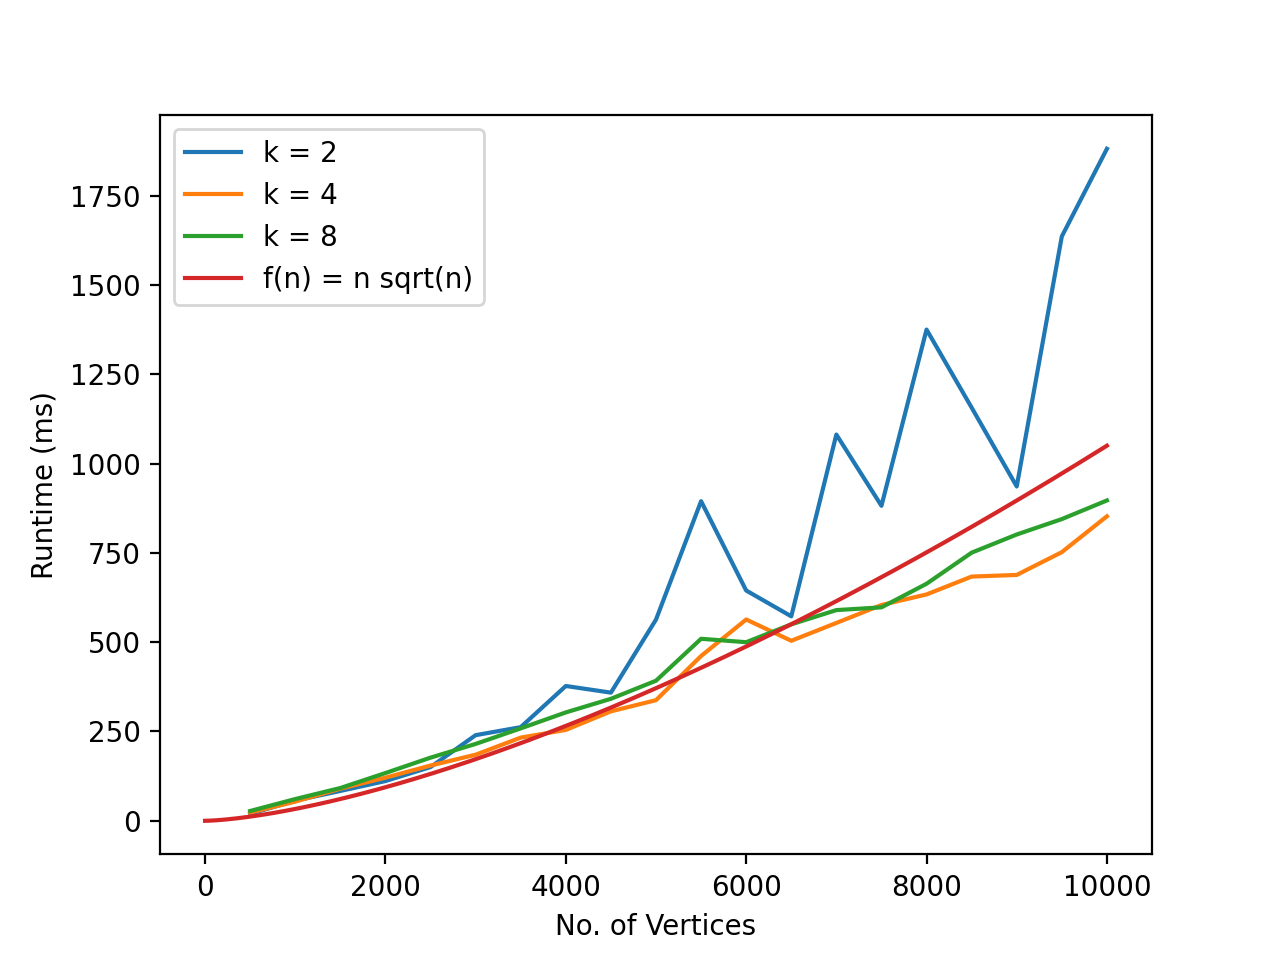
\includegraphics[width=0.9\linewidth, height=7cm]{pic/ch-Exp/kin_time.png}
\caption{Runtime plot of $D_{k-in, k-out}$}
\label{fig:kin:time}
\end{subfigure}
\begin{subfigure}{\textwidth}
\centering
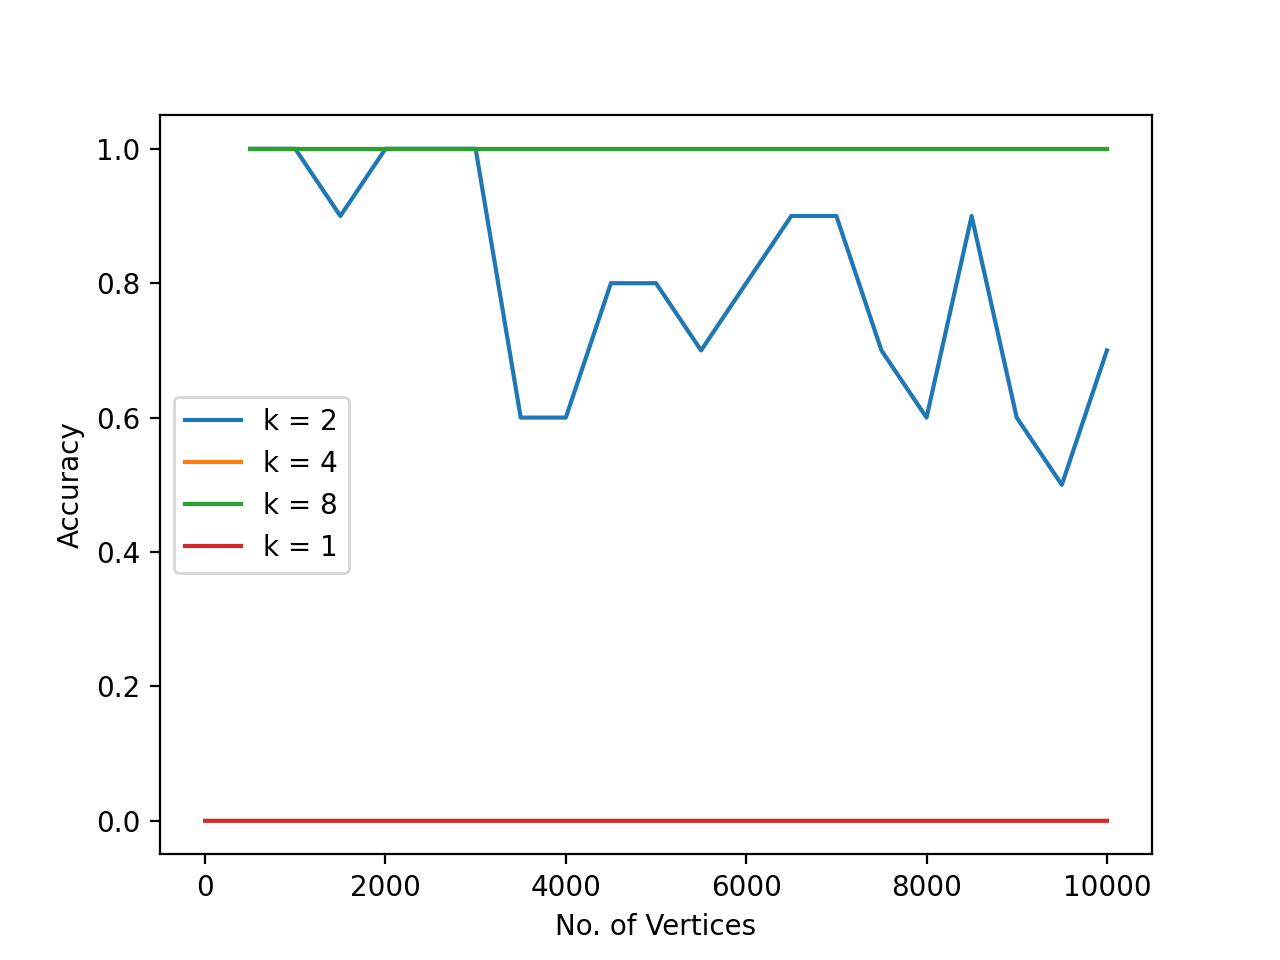
\includegraphics[width=0.9\linewidth, height=7cm]{pic/ch-Exp/kin_accr.png}
\caption{Probability of finding a Hamilton cycle in $D_{k-in, k-out}$}
\label{fig:kin:accr}
\end{subfigure}

\caption{DHAM on $D_{k-in, k-out}$}
\label{fig:kin:plots}
\end{figure}

We try to test if DHAM might be successful in finding this Hamiltonian cycle in polynomial time.
From \autoref{fig:kin:time} we can see that (to the extend of n that is feasible for testing)
that runtime grows more or less the same as on $D_{n, m}$. This is suggestive of the fact that it might be possible to give a polynomial bound the runtime of 3-phase method on this class of graphs. 

We also see some spikes in the runtime and also a lower probability of finding the Hamiltonian cycle in \autoref{fig:kin:accr} for $D_{2-in, 2-out}$, even though we know that this graph is Hamiltonian with high probability. This phenomenon is observed again in the next model we take a look at and seems to suggest that the algorithm does not run as well on sparse graphs. 


\section{$k$-regular Graphs}
\subsection{Graph Generation}
To generate a $k$-regular digraph, we need to make sure that the in-degree and the out-degree of each vertex are k. But simply choosing $2k$ neighbours independently like for $D_{k-in, k-out}$ does not work, since we cannot guarantee that exactly $k$ other vertices will also be in-neighbours.

Instead, we notice that in a permutation digraph, each vertex has exactly $1$ in/out neighbour. We use this fact and take the union of k random permutation digraphs (which have no mutual overlap) to obtain a $k$-regular digraph.
\subsection{Observations}
Theoretically, it has been shown that $D_{n, r}$ is Hamiltonian with high probability for $r \ge 3$ \cite{cooper:kreg}. The proof for this is again based on a 3-phase method and is very similar to that for $D_{k-in, k-out}$, since large $k$-regular graphs look very similar to $D_{k-in, k-out}$ graphs. Hence it is not very surprising that their runtime plots look similar. The runtime very closely follows the same $n^{1.5}$ curve that $D_{n, m}$ had, suggesting that it might be possible to give a polynomial bound for DHAM on this class of graphs too.

Once again we notice the spikes in runtime and the lower probabilities of success for $k = 2, 3$ in \autoref{fig:kreg:accr}, reiterating the idea that DHAM performs poorly on sparse graphs. We can trace this bad performance to the first phase of the algorithm, where we construct a subgraph of average degree 10. The bipartite matching that follows depends on the degree of vertices in this subgraph, and a lower degree limits the success probability of the matching, and hence bottle-necking DHAM. 

\begin{figure}[ht]

\begin{subfigure}{\textwidth}
\centering
\includegraphics[width=0.9\linewidth, height=7cm]{pic/ch-Exp/kreg_time.png}
\caption{Runtime plot of $D_{n, r}$}
\label{fig:kreg:time}
\end{subfigure}
\begin{subfigure}{\textwidth}
\centering
\includegraphics[width=0.9\linewidth, height=7cm]{pic/ch-Exp/kreg_accr.png}
\caption{Probability of finding a Hamilton cycle in $D_{n, r}$}
\label{fig:kreg:accr}
\end{subfigure}

\caption{DHAM on $D_{n, r}$}
\label{fig:kreg:plots}
\end{figure}
\subsection{Closer look at sparse graphs}
Since we notice the DHAM performs poorly on sparse graphs, but still works just fine at value below the mentioned degree $10$, in the original paper, we take a closer look to see above what value of $r$, does DHAM find a cycle in $D_{n, r}$, with high probability and low number of attempts.

\begin{figure}[ht]

\begin{subfigure}{\textwidth}
\centering
\includegraphics[width=0.9\linewidth, height=7cm]{pic/ch-Exp/sprc_accr.png}
\caption{Probability of Finding a cycle in sparse $D_{n, r}$}
\label{fig:kreg:spaccr}
\end{subfigure}
\begin{subfigure}{\textwidth}
\centering
\includegraphics[width=0.9\linewidth, height=7cm]{pic/ch-Exp/sprc_atmp.png}
\caption{Average no. of attempts to find the cycle}
\label{fig:kreg:spatmp}
\end{subfigure}

\caption{$D_{n, r}$ with low values of $r$}
\label{fig:kreg:sparse}
\end{figure}

From \autoref{fig:kreg:sparse} we see that for $r \ge 6$, the probability of finding a cycle is almost at 1, and the number of attempts also stabilises around 5. 

\section{Random Tournaments}
\subsection{Graph Generation}
We can generate every possible pair of vertices, using a nested loop, and assign a direction to every edge uniformly at random to obtain the desired tournament.
\subsection{Observations}
Random Tournaments have been shown to have $\delta = min(\delta^+, \delta^-)$ edge disjoint Hamiltonian cycles\cite{kuhn:tourna}. Though the proof does not rely on the 3-phase method, DHAM using that method, still does find cycles in such graphs (\autoref{fig:tourna:time}), with high probability (probability 1 in our tests).

Tournaments grow in size as a function of $n^2$, limiting the range of $n$ feasible for testing. From the range of sizes that we tested on it is not possible to comment on the runtime on these graphs (since the implementation overhead might be affecting the runtime more than the algorithm itself). But we do notice that every graph generated returned a valid Hamiltonian cycle, which seems to suggest that the probability of success of the 3-phase method is also very high on random tournaments.
Also, since tournaments are dense graphs, we do not run into the bottlenecks that we observed in the last 2 models.

\begin{figure}[ht]

\centering
\includegraphics[width=0.9\linewidth,height=7cm]{pic/ch-Exp/tourna_time.png}
\caption{Runtime plot of Tournaments}
\label{fig:tourna:time}

\end{figure}

\section{Random $n$-lifts of complete digraph $K_h$}
\subsection{Graph Generation}
We first create the complete digraph, $K_h$ on $h$ vertices. Now, we start constructing a new digraph $D$, with $h \times n$ vertices, with the range of vertices $[i \times n, i \times (n+1) - 1]$ corresponding to each vertex $i\in V(K_h)$. 

Now, for each edge $(u, v) \in E(K_h)$, we construct arrays $U$ \& $V$, of the vertices corresponding to $u, v \in V(K_h)$. After shuffling the arrays, we obtain a random matching as $\forall i<n, (U[i], V[i])$, which is now added to the graph $D$, to obtain the required $n$-lift of $K_h$.
\subsection{Observations}
This is another class of graphs that proved to be Hamiltonian \cite{frieze:lift} (for sufficiently large values of $h$) by using the 3-phase method, with appropriate modifications.
\begin{description}
\item[Phase 1] Show that with high probability the lift $D$ contains a directed permutation digraph, $\Pi$ of size at most $2\ln n$.
\item[Phase 2] Increase the minimum cycle length in $\Pi$ to $n_0 = \Big\lceil \frac{100nh^3}{\ln n} \Big\rceil$.
\item[Phase 3] Convert the Phase 2 permutation digraph to a Hamilton Cycle.
\end{description}

We make some interesting observations here. 
The first is that for $k=8$ we see that all the generated graphs are Hamiltonian, which could be considered a more precise lower bound for $h$ than the \textit{sufficiently large h} . But more importantly, none of the n-lifts of $K_3$ are Hamiltonian. Frieze in his survey\cite{frieze:2019survey}, has posed the problem to show that n-lifts of $K_3$ are Hamiltonian. What we observe with DHAM, is that the probability of lifts of $K_3$ being Hamiltonian is zero. Though this particular algorithm failing, need not imply that n-lifts of $K_3$ are not Hamiltonian (indeed it could be because of the phenomenon of DHAM doing poorly on sparse graphs, with us also observing the runtime spikes, and low probability at $k=4$), it is an interesting observation nevertheless and worth taking a deeper look into.

\begin{figure}[ht]

\begin{subfigure}{\textwidth}
\centering
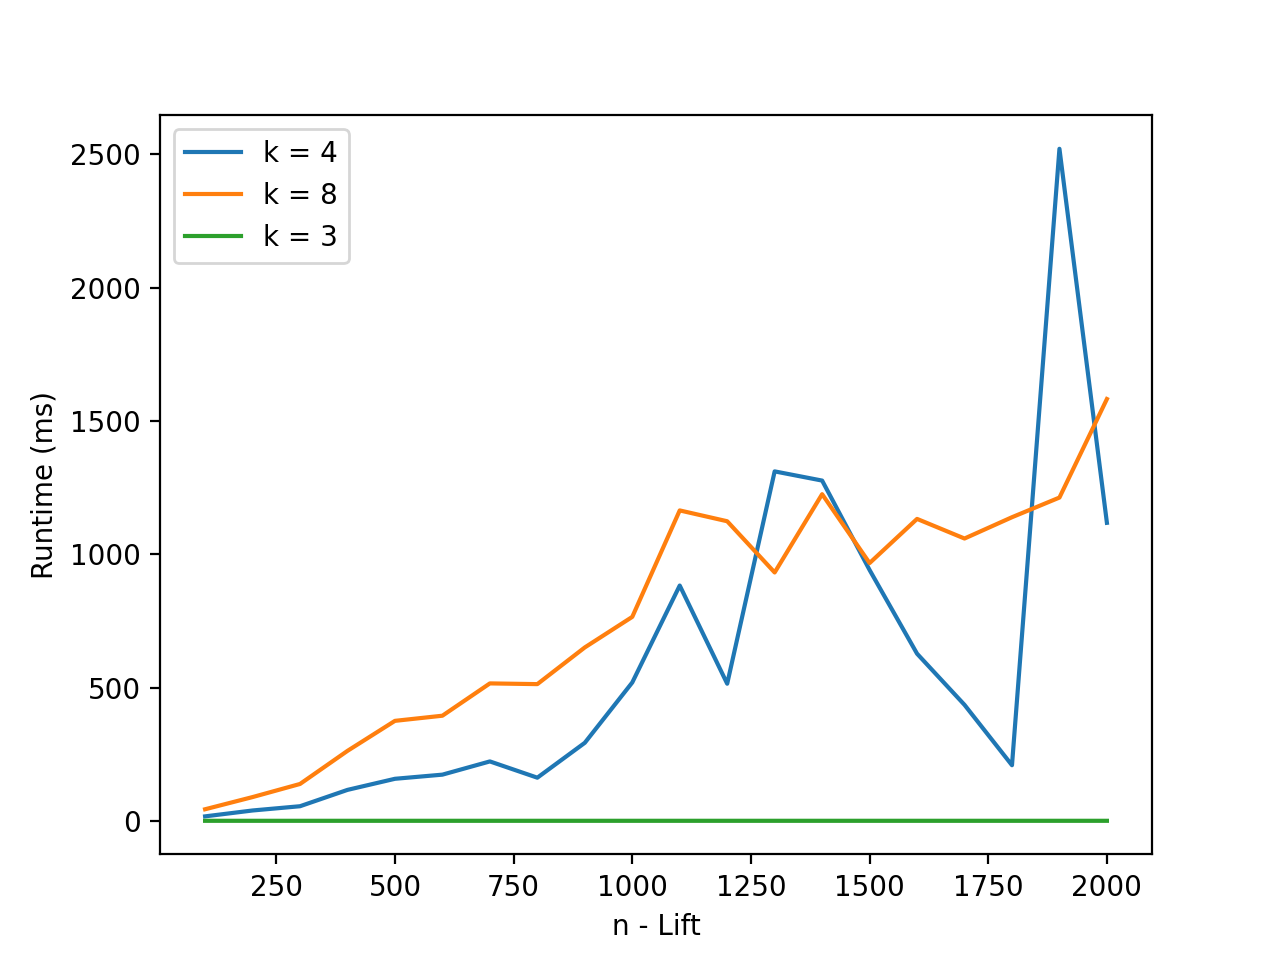
\includegraphics[width=0.9\linewidth,height=7cm]{pic/ch-Exp/nlift_time.png}
\caption{Runtime plot of n-lifts}
\label{fig:nlift:time}
\end{subfigure}
\begin{subfigure}{\textwidth}
\centering
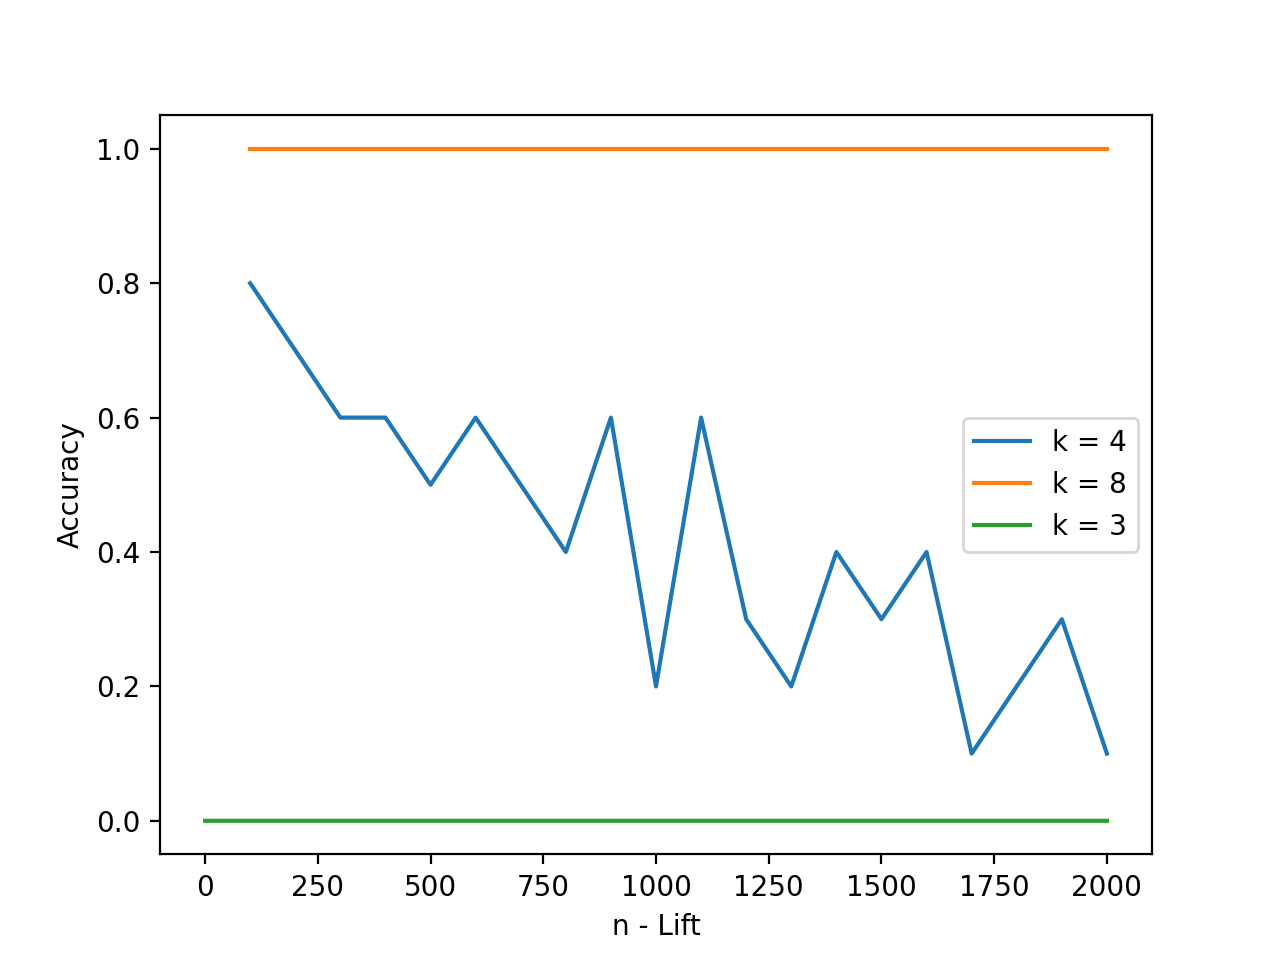
\includegraphics[width=0.9\linewidth, height=7cm]{pic/ch-Exp/nlift_accr.png}
\caption{Probability of finding a Hamilton cycle in lifts of $K_h$}
\label{fig:lift:accr}
\end{subfigure}

\caption{DHAM on n-lifts}
\label{fig:other:plots}
\end{figure}